\documentclass[UTF-8,twoside,cs4size]{ctexart}
\usepackage{amsmath}
\usepackage{amssymb}
\usepackage{geometry}
\usepackage{setspace}
\usepackage{xeCJK}
\usepackage{ulem}
\usepackage{pstricks}
\usepackage{pstricks-add}
\usepackage{bm}
\usepackage{mathtools}
\usepackage{breqn}
\usepackage{mathrsfs}
\usepackage{esint}
\usepackage{textcomp}
\usepackage{upgreek}
\usepackage{pifont}
\usepackage{tikz}
\usepackage{circuitikz}
\usepackage{caption}
\usepackage{xcolor}
\usepackage{tabularx}
\usepackage{array}
\usepackage{pgfplots}
\usepackage{multirow}
\usepackage{pgfplotstable}

\newcolumntype{Y}{>{\centering\arraybackslash}X}
\geometry{a4paper,centering,top=0.75cm,bottom=2.54cm,left=2cm,right=2cm}
\pagestyle{plain}
\captionsetup{font=small}

%\CTEXsetup[name={,.}]{section}
\CTEXsetup[format={\raggedright\bfseries\noindent\zihao{3}}]{section}
\CTEXsetup[format={\raggedright\bfseries\quad\large}]{subsection}
\CTEXsetup[format={\raggedright\bfseries\qquad}]{subsubsection}
\renewcommand\thefootnote{\ding{\numexpr171+\value{footnote}}}

\setstretch{1.5}

\setCJKfamilyfont{boldsong}[AutoFakeBold = {2.17}]{SimSun}
\newcommand*{\boldsong}{\CJKfamily{boldsong}}
%\DeclareMathOperator\dif{d\!}
\newcommand*{\me}{\mathop{}\!\mathrm{e}}
\newcommand*{\mpar}{\mathop{}\!\partial}
\newcommand*{\dif}{\mathop{}\!\mathrm{d}}
\newcommand*{\tab}{\indent}

\begin{document}
	\begin{flushright}
		\zihao{2}{分组号:3-07}
	\end{flushright}
	
	\noindent{\zihao{-2}\boldsong\bfseries 《\,\, 基\,\, 础\,\, 物\,\, 理\,\, 实\,\, 验\,\, 》\,\, 实\,\, 验\,\, 报\,\, 告\,\, }
	
	\noindent\textit{实验名称\uline{\quad\qquad\qquad\quad\qquad\qquad 驻波实验\,\qquad\qquad\qquad\qquad\qquad}指导教师\uline{\qquad\,\,\,边勇波\,\,\,\qquad}}
	
	\noindent\textit{姓\qquad 名\uline{\,\,\, 桂庭辉\,\,\,}\,学号\uline{\,\,\,{\upshape2019K8009929019}\,\,\,}\,专\qquad 业\uline{\,\,\,计算机科学与技术\,\,\,}\,班级\uline{\,\,\,\upshape{03}\,\,\,}\,座号\uline{\,\,\,\upshape{6}\,\,\,}}
	
	\noindent\textit{实验日期\uline{\,\,{\upshape 2020}\,\,}年\uline{\,\,{\upshape 12}\,\,}月\uline{\,\,{\upshape09}\,\,}日\,\,实验地点\uline{\,\,\,教学楼{\upshape721}\,\,\,}调课/补课\uline{\,\,\,$ \square $是\,\,\,}成绩评定\uline{\,\,\,\quad\qquad\qquad}}
	
	\begin{table}[h]
		\centering
		\psset{linewidth=2pt}
		\begin{pspicture}(-1,-0.1)(1,0.1)
		\psline(-9,0)(9,0)
		\end{pspicture}
	\end{table}
	\begin{center}
		\Large\bfseries 第一部分\quad 弦上驻波实验
	\end{center}
	\section{实验目的}
	1.观察在两端固定的弦线上形成的驻波现象,了解弦线达到共振和形成稳定驻波的条件;
	
	2.测定弦线上横波的传播速度;
	
	3.用实验的方式确定弦线作受迫振动时共振频率和半波长个数$ n $、弦线有效长度、张力及线密度之间的关系;
	
	4.用对数作图和最小二乘法对共振频率与张力关系的实验结果作线性拟合,处理数据,并给出结论。
	
	\section{实验器材}
	本实验主要实验装置有弦音计、信号发生器、双踪示波器三部分。此外还有天平等测量工具。
	
	1.弦音计由吉他弦、固定吉他弦的支架和基座、琴码、砝码支架、驱动线圈、探测线圈和砝码等组成。驱动线圈和探测线圈是本装置的重要部分,其中驱动线圈通过信号发生器提供一定频率的功率信号产生交变磁力,使得金属弦线振动;探测线圈将弦线的振动转换为电信号,通过示波器进行观察。
	
	\begin{figure}[!h]
		\centering
		\begin{tikzpicture}
			\filldraw[black,fill opacity=0.5] (0,1)--(0.7,1)--(0.9,0.8)--(1.1,0.8)--(1.3,1)--(1.7,1)--(1.9,0.8)--(2.1,0.8)--(2.3,1)--(2.7,1)--(2.9,0.8)--(3.1,0.8)--(3.3,1)--(3.7,1)--(3.9,0.8)--(4.1,0.8)--(4.3,1)--(4.7,1)--(4.9,0.8)--(5.1,0.8)--(5.3,1)--(6,1)--(6,0.5)--(0,0.5)--(0,1)--cycle;
			\draw[dashed] (1,1.5)--(1,-0.5);
			\draw[dashed] (2,2)--(2,-0.5);
			\draw[dashed] (3,2.5)--(3,-0.5);
			\draw[dashed] (4,3)--(4,-0.5);
			\draw[dashed] (5,3.5)--(5,-0.5);
			\draw[dashed] (0.7,-1) rectangle (1.3,-0.5);
			\draw[dashed] (1.7,-1) rectangle (2.3,-0.5);
			\draw[dashed] (2.7,-1) rectangle (3.3,-0.5);
			\draw[dashed] (3.7,-1) rectangle (4.3,-0.5);
			\draw[dashed] (4.7,-1) rectangle (5.3,-0.5);
			\node[below left] at(1,0.5) {1};
			\node[below left] at(2,0.5) {2};
			\node[below left] at(3,0.5) {3};
			\node[below left] at(4,0.5) {4};
			\node[below left] at(5,0.5) {5};
			\draw[->] (1,1.5)--(1.6,1.5) node[right]{$ 1mg $};
			\draw[->] (2,2)--(3.2,2) node[right]{$ 2mg $};
			\draw[->] (3,2.5)--(4.8,2.5) node[right]{$ 3mg $};
			\draw[->] (4,3)--(6.4,3) node[right]{$ 4mg $};
			\draw[->] (5,3.5)--(8,3.5) node[right]{$ 5mg $};
			\draw (-4,-1) rectangle (0,3);
			\node at(-2,1) {弦音计};
		\end{tikzpicture}
		\caption{弦音计砝码在不同槽位对弦线的拉力}
	\end{figure}
	
	2.信号发生器为低频功率信号发生器,其输出信号的频率从$ 10\,\mathrm{Hz} $到$ 1\,\mathrm{kHz} $,用于为驱动线圈提供上述频率范围中具有一定功率的正弦信号。
	
	3.双踪示波器用于观察信号源的波形并显示由探测线圈接收到的弦线振动的波形,进而可以及时观察弦线的振动现象。
	
	\section{实验原理}
	将一弦线两端固定,在一端附近使得弦线作振幅恒定的连续简谐振动,从而将有连续的横波波列从该端向另一端传播,前进波传播到另一端时即会发生反射,回到原端点时再次反射,如此不断重复下去。弦线上既有前进波,又有无数的反射波。如果弦线的长度与波长之间满足某种关系,使得前进波与许多反射波都具有相同的相位时,弦线上各点作振幅各自恒定的简谐振动。那么弦线上有些点振动振幅最大,成为波腹;有些点的振幅为零,成为波节,形成驻波现象。
	
	\begin{figure}[!h]
		\centering
		\begin{tikzpicture}
			\draw [domain=0:4*pi,samples=1000,thick] plot (\x,{sin(2*\x r)});
			\draw [domain=0:4*pi,samples=1000,thick,dashed] plot (\x,{-sin(2*\x r)});
			\draw [->] (pi,-2.5)node[below]{波节}--(pi,-0.5);
			\draw [->] (2.75*pi,-2.5)node[below]{波腹}--(2.75*pi,-1.2);
			\draw [ultra thick] (0,-1.2)--(0,1.2);
			\draw [ultra thick] (4*pi,-1.2)--(4*pi,1.2);
		\end{tikzpicture}
		\caption{驻波现象示意图}
	\end{figure}
	
	相邻两波节(或波腹)的间隔距离$ D $为波长$ \lambda $的一半,称为半波长,即$ D=\frac\lambda2 $。由于弦线两端固定,故而弦线两端均为波节,那么弦线长度应为半波长的整数倍,记弦线长度为$ L $,则
	\[L=nD=\frac{n\lambda}{2},\qquad n=1,2,3,\cdots\]
	
	设振动频率为$ f $,则横波沿弦线的传播速度为$ v=f\lambda $。根据波动理论,记拉紧的弦上张力为$ T $,弦线线密度为$ \mu $,波在传播方向的位置坐标为$ x $,振动位移为$ y $,那么沿弦线传播的横波应满足:
	\[\frac{\mpar^2y}{\mpar t^2}=\frac{T\mpar^2y}{\mu\mpar x^2},\qquad\frac{\mpar^2y}{\mpar t^2}=v^2\frac{\mpar^2y}{\mpar x^2}\]
	进而可以得到波的传播速度满足
	\[v=\sqrt{\frac T\mu}\]
	对比其与$ v=f\lambda $之间的差异,分析理论值与测量值间的区别。
	
	此外频率与张力、线密度间的关系可求得为
	\[f=\frac1\lambda\sqrt{\frac T\mu}\]
	对上式两边取对数,则有
	\[\ln f=\frac12\ln T-\frac12\ln\mu-\ln\lambda\]
	
	\section{实验内容}
	1.认识和调节仪器;
	
	2.测定所用弦线的线密度。用天平测定弦线\footnote{选用与所用弦线直径相同、只取吉他弦中段约70-80\,cm的专用样品,而非从弦音计上取下弦线进行测量。}的质量$ m $,并测量弦线长$ L $,则线密度为
	\[\mu=\frac mL\]
	
	3.观察弦线上的驻波。固定弦上张力$ T $与波的有效长度$ L $,调节信号发生器的输出频率,观察在两端固定的弦线上形成的有$ n\;(n=1,2,3,\cdots) $个波腹的稳定驻波。
	
	4.测定弦线上横波的传播速度。(1)测得张力$ T $与线密度$ \mu $,根据$ v=\sqrt{\frac T\mu} $测得横波传播速度。(2)测出共振频率$ f $,波的有效长度$ L $,根据$ \lambda=\frac{2L}{n} $求得波长,再利用$ v=\lambda f $计算得到横波传播速度。比较两种方法得到的实验结果。
	
	5.固定弦线线密度与弦线张力,确定弦线作受迫振动时的共振频率(只取基频,即$ n=1 $)与弦线有效长度之间的关系,并记录数据。
	
	6.固定弦线线密度与弦线有效长度,确定弦线作受迫振动时的共振频率(只取基频,即$ n=1 $)与张力之间的关系,并记录数据。
	
	7.固定弦线张力、弦线有效长度,确定弦线作受迫振动时的共振频率(只取基频,即$ n=1 $)与弦线线密度之间的关系,并记录数据。
	
	\section{实验结果与数据处理}
	\subsection{线密度测定}
	\begin{table}[!h]
		\centering
		\renewcommand\arraystretch{1.5}
		\caption{所用弦线线密度的测定}
		\begin{tabularx}{\textwidth}{|c|Y|Y|Y|Y|}
			\hline
			\textbf{弦号}&\textbf{质量}(g)&\textbf{长度}(mm)&\textbf{直径}(mm)&\textbf{线密度}(kg/m)\\
			\hline
			6&0.059&58.75&0.410&0.0010\\
			\hline
		\end{tabularx}
	\end{table}
	虽与线密度测量无关,但后续实验探究频率与线密度关系时,需使用不同粗细琴弦得到的结果,故测量直径以便区分各弦。
	\subsection{波速的测量}
	将琴码放置于150\,mm和650\,mm处,则弦线有效长度$ L=500\,\mathrm{mm} $,不同频率$ f_n\,(n=1,2,3) $对应的波长$ \lambda=\frac{2L}{n} $,故而$ f_1,f_2,f_3 $对应波速公式分别为$ v_1=2Lf_1,\,v_2=Lf_2,\,v_3=\frac{2Lf_3}{3} $,测得波速所用数据如下:	
	\begin{table}[!h]
		\centering
		\renewcommand\arraystretch{1.5}
		\caption{根据$ v=\lambda f $测量波速}
		\begin{tabularx}{\textwidth}{|c|Y|Y|Y|Y|Y|Y|Y|}
			\hline
			\textbf{砝码位置}$ k $&$ f_1\,(\mathrm{Hz}) $&$ v_1\,(\mathrm{m/s}) $&$ f_2(\mathrm{Hz}) $&$ v_2\,(\mathrm{m/s}) $&$ f_3(\mathrm{Hz}) $&$ v_3\,(\mathrm{m/s}) $&$ \bar v\,(\mathrm{m/s}) $\\
			\hline
			2&70.9&70.90&142.5&71.25&214.0&71.33&71.16\\
			\hline
			3&90.9&90.90&179.5&89.75&269.7&89.90&90.18\\
			\hline
			4&102.2&102.20&203.9&101.95&305.2&101.73&101.96\\
			\hline
		\end{tabularx}
	\end{table}

	由于弦右端受到大小为$ kmg\,(k=2,3,4) $的拉力,故而弦上张力$ T=\frac12kmg $。实验测得砝码质量$ m=508.40\,\mathrm g $,再根据$ v=\sqrt{\frac T\mu} $可计算得到波速、其与根据$ v=\lambda f $得到的$ \bar v $之间的相对误差如下表:
	\begin{table}[!h]
		\centering
		\renewcommand\arraystretch{1.5}
		\caption{根据$ v=\sqrt{\frac T\mu} $测量波速}
		\begin{tabularx}{\textwidth}{|c|Y|Y|Y|Y|}
			\hline
			\textbf{砝码位置}$ k $&$ T\,(\mathrm N) $&$ v\,(\mathrm{m/s}) $&$ \bar v\,(\mathrm{m/s}) $&\textbf{相对误差}\,\%\\
			\hline
			2&4.982&70.58&71.16&0.815\\
			\hline
			3&7.473&86.45&90.18&4.136\\
			\hline
			4&9.965&99.92&101.96&2.001\\
			\hline
		\end{tabularx}
	\end{table}

	可见在误差允许范围内两种方法得到的波速大小可看作相等。
	
	\begin{figure}[!h]
		\centering
		\includegraphics*[scale=0.1]{5-2.jpg}
		\caption{实验中观察到的波节}
	\end{figure}
	
	\subsection{频率与有效长度的关系}
	将砝码勾在第2格,改变有效长度,测量基频$ f_1 $,数据实验数据如下:
	\begin{table}[!h]
		\centering
		\renewcommand\arraystretch{1.5}
		\caption{不同有效长度下的基频}
		\begin{tabularx}{\textwidth}{|c|Y|Y|Y|Y|Y|}
			\hline
			$ L\,(\mathrm{m}) $&0.640&0.480&0.320&0.240&0.160\\
			\hline
			$ f_1\,(\mathrm{Hz}) $&54.1&72.7&116.7&155.9&235.5\\
			\hline
			$ \ln L $&$ -0.446 $&$ -0.734 $&$ -1.139 $&$ -1.427 $&$ -1.833 $\\
			\hline
			$ \ln f_1 $&3.991&4.286&4.760&5.049&5.462\\
			\hline
		\end{tabularx}
	\end{table}

	根据上表数据可作出上图拟合直线。
	\begin{figure}[!h]
		\centering
		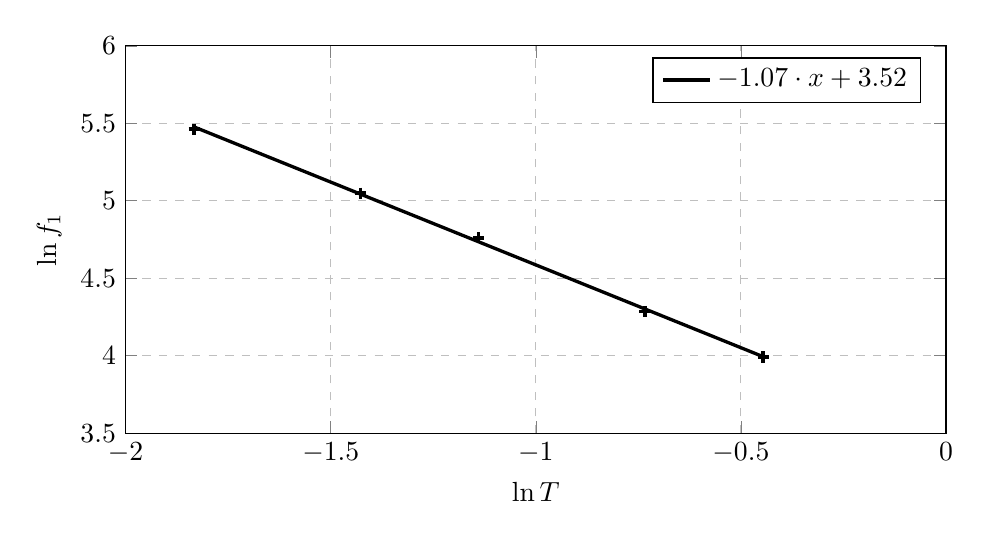
\begin{tikzpicture}
			\begin{axis}[
				legend pos=north east,
				width=12cm,height=6.5cm,
				xlabel=$ \ln T $,
				ylabel=$ \ln f_1 $,
				xmin=-2,xmax=0,
				ymin=3.5,ymax=6,
				xtick={-2,-1.5,-1,-0.5,0},
				ytick={3.5,4,4.5,5,5.5,6},
				grid style=dashed,
				ymajorgrids=true,
				xmajorgrids=true,
				]
				\addplot[no marks,black,very thick] table[y={create col/linear regression={y=Y}}]
				{
					X	Y
					-0.446	3.991
					-0.734	4.286
					-1.139	4.760
					-1.427	5.049
					-1.833	5.462			
				};
				\addlegendentry{
					$\pgfmathprintnumber{\pgfplotstableregressiona} \cdot x
					\pgfmathprintnumber[print sign]{\pgfplotstableregressionb}$}
				
				\addplot [very thick,mark=+,only marks] coordinates {
					(-0.446,3.991)(-0.734,4.286)(-1.139,4.760)(-1.427,5.049)(-1.833,5.462)
				};
			\end{axis}
		\end{tikzpicture}
		\captionsetup{skip=0pt}
		\caption{$ \ln f_1-\ln T $拟合直线}
	\end{figure}

	由拟合直线斜率$ k=-1.07\approx-1 $可知在误差允许范围内可认为$ \ln f_1=-\ln L+C $(此时$ C $为常数),即$ f_1\propto\frac1L $,又由于$ L\propto\lambda $,故而实际验证的物理规律为$ f_1\propto\lambda_1 $.

%	理论上上表第三行中数据应在误差允许范围内可看作相等,但实际数据中前两项相等,后三项相等,可能的原因是当弦线有效长度减小后,激振源与接收器距离过近,激振源发出信号由接收器直接接收对基频的测定造成了干扰使得实验结果出错。
	
	\subsection{频率与张力的关系}
	将琴码分别放置在200\,mm和600\,mm位置,固定有效长度$ L=400\,\mathrm{mm} $,将砝码分别放置在1-5格,测量不同拉力下的基频$ f_1 $。数据记录如下:
	\begin{table}[!h]
		\centering
		\renewcommand\arraystretch{1.5}
		\caption{不同拉力下的基频}
		\begin{tabularx}{\textwidth}{|c|Y|Y|Y|Y|Y|}
			\hline
			\textbf{位置}&\textbf{1}&\textbf{2}&\textbf{3}&\textbf{4}&\textbf{5}\\
			\hline
			$ T\,(\mathrm{N}) $&2.491&4.982&7.473&9.965&12.456\\
			\hline
			$ \ln T $&0.913&1.606&2.011&2.299&2.522\\
			\hline
			$ f_1\,(\mathrm{Hz}) $&62.5&87.9&112.6&127.7&143.3\\
			\hline
			$ \ln f_1 $&4.135&4.476&4.724&4.850&4.965\\
			\hline
		\end{tabularx}
	\end{table}
	
	根据上表数据可作出拟合图象如图(\ref{f-t})。由拟合直线斜率$ k=0.52\approx\frac12 $可知$ \ln f_1=\frac 12\ln T+C $(此时$ C $为常数),即$ f_1\propto\sqrt{T} $.
	
	\begin{figure}[!h]
		\centering
		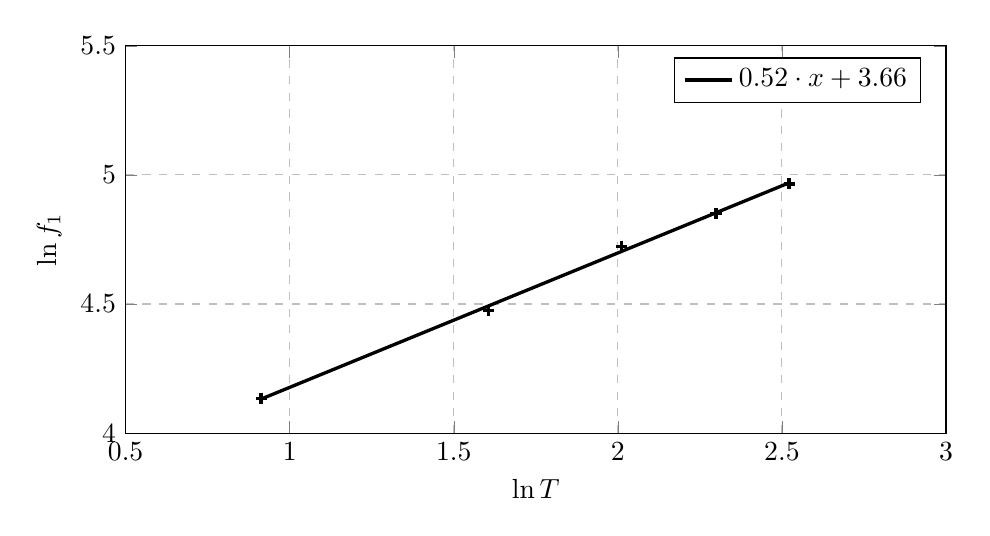
\begin{tikzpicture}
			\begin{axis}[
				legend pos=north east,
				width=12cm,height=6.5cm,
				xlabel=$ \ln T $,
				ylabel=$ \ln f_1 $,
				xmin=0.5,xmax=3,
				ymin=4,ymax=5.5,
				xtick={0.5,1,1.5,2,2.5,3},
				ytick={4,4.5,5,5.5},
				grid style=dashed,
				ymajorgrids=true,
				xmajorgrids=true,
				]
				\addplot[no marks,black,very thick] table[y={create col/linear regression={y=Y}}]
				{
					X	Y
					0.913	4.135
					1.606	4.476
					2.011	4.724
					2.299	4.850
					2.522	4.965			
				};
				\addlegendentry{
					$\pgfmathprintnumber{\pgfplotstableregressiona} \cdot x
					\pgfmathprintnumber[print sign]{\pgfplotstableregressionb}$}
				
				\addplot [very thick,mark=+,only marks] coordinates {
					(0.913,4.135)(1.606,4.476)(2.011,4.724)(2.299,4.850)(2.522,4.965)
				};
			\end{axis}
		\end{tikzpicture}
		\caption{$ \ln f_1-\ln T $拟合直线图象}
		\label{f-t}
	\end{figure}
	
	\subsection{频率与线密度之间的关系}
	将琴码分别放置在200\,mm和600\,mm位置,固定有效长度$ L=400\,\mathrm{mm} $,将砝码放置在第2格,通过共享数据得到不同粗细琴弦的基频。数据记录如下:
	\begin{table}[!h]
		\centering
		\renewcommand\arraystretch{1.5}
		\caption{不同粗细琴弦的基频}
		\begin{tabularx}{\textwidth}{|Y|Y|Y|Y|Y|}
			\hline
			\textbf{弦号}&5&6&7&8\\
			\hline
			\textbf{直径}(mm)&0.601&0.410&0.85&1.06\\
			\hline
			\textbf{线密度}$\mu$(kg/m)&0.0018&0.0010&0.0035&0.0057\\
			\hline
			\textbf{基频}$ f_1 $(Hz)&64.6&87.9&49.3&37.3\\
			\hline
			$ \ln\mu $&$ -6.320 $&$ -6.908 $&$ -5.655 $&$ -5.167 $\\
			\hline
			$ \ln f_1 $&4.168&4.476&3.898&3.619\\
			\hline
		\end{tabularx}
	\end{table}
	
	由上表数据可作出如下拟合图象:
	\begin{figure}[!h]
		\centering
		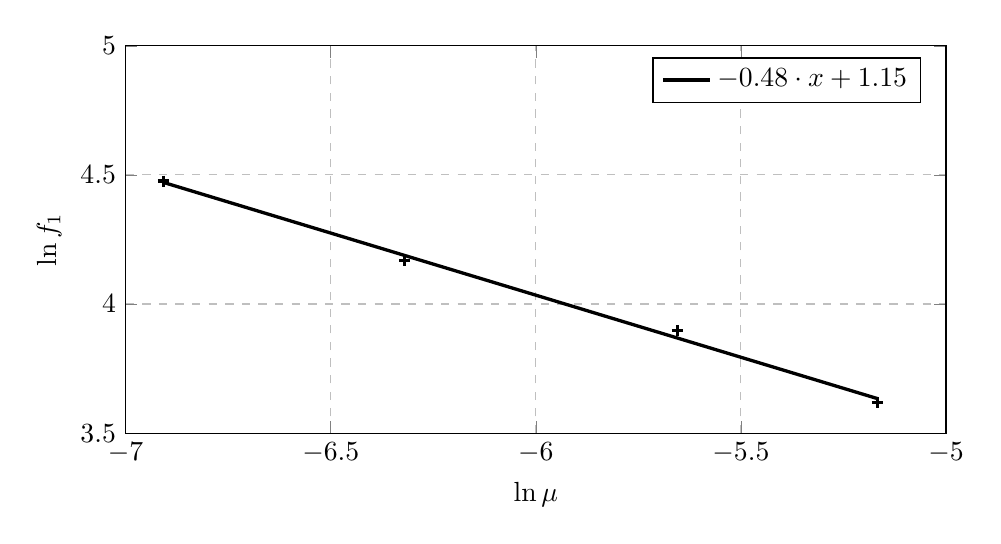
\begin{tikzpicture}
			\begin{axis}[
				legend pos=north east,
				width=12cm,height=6.5cm,
				xlabel=$ \ln \mu $,
				ylabel=$ \ln f_1 $,
				xmin=-7,xmax=-5,
				ymin=3.5,ymax=5,
				xtick={-7,-6.5,-6,-5.5,-5},
				ytick={3.5,4,4.5,5},
				grid style=dashed,
				ymajorgrids=true,
				xmajorgrids=true,
				]
				\addplot[no marks,black,very thick] table[y={create col/linear regression={y=Y}}]
				{
					X	Y
					-6.908	4.476
					-6.320	4.168
					-5.655	3.898
					-5.167	3.619			
				};
				\addlegendentry{
					$\pgfmathprintnumber{\pgfplotstableregressiona} \cdot x
					\pgfmathprintnumber[print sign]{\pgfplotstableregressionb}$}
				
				\addplot [very thick,mark=+,only marks] coordinates {
					(-6.908,4.476)(-6.32,4.168)(-5.655,3.898)(-5.167,3.619)
				};
			\end{axis}
		\end{tikzpicture}
		\caption{$ \ln f_1-\ln\mu $拟合直线}
	\end{figure}
	
	由拟合直线斜率$ k=-0.48\approx-\frac12 $可知$ \ln f_1=-\frac12\ln\mu+C $(此时$ C $为常数),即$ f_1\propto\frac{1}{\sqrt \mu} $.
	
	\section{实验总结}
	\subsection{思考题}
	1.调节振动源上的振动频率和振幅大小后对弦线振动会产生什么影响?
	
	{\kaishu 弦线的振动由振动源的振动引起。若调节振动源的频率,则会影响弦线上各点处前进波与反射波的干涉情况,一定条件下,驻波现象产生;调节振动源振幅大小,将影响弦线上各点的振动振幅,但对驻波现象是否产生没有影响。}
	
	~\
	
	2.如何来确定弦线上的波节点位置?
	
	{\kaishu 粗略观察可直接由肉眼观察弦线上几乎没有振幅(即振幅为0)的点,即为波节点。}
	
	{\kaishu 若需较为精确地寻找到波节,则可通过调节接收器的位置,观察示波器上接收到的波形,接收器移动过程中观察到的波形振幅最小处即为波节点。}
	
	~\
	
	3.在弦线上出现驻波的条件是什么?在实验中为什么要把弦线的振动调到驻波现在最稳定、最显著的状态?
	
	{\kaishu 根据实验原理部分可知出现驻波的条件为$ n\lambda = 2L\;(n=1,2,3,\cdots) $,即有效长度是半波长的正整数倍。将弦线振动调节至驻波最稳定、最显著时弦线状态最接近驻波出现条件的状态,确保各点处前进波和反射波确实发生了有稳定相位差的稳定干涉,使得测得的基频更为准确。}
	
	4.在弹奏弦线乐器时,发出声音的音调与弦线的长度、粗细、松紧程度由什么关系?为什么?
	
	{\kaishu 在弹奏弦线乐器时,弦线长度越短\footnote{长度$ L $与相应驻波波长$ \lambda $成正相关。}、直径越小\footnote{直径越小的弦线线密度小。}、琴弦越紧\footnote{即弦线上拉力$ T $更大。},发出声音的音调越高。弦线乐器的声音与弦线振动的频率$ f $正相关,而由实验过程验证过的实验原理$ \ln f=\frac12\ln T-\frac12\ln\mu-\ln\lambda $可得:$ f\propto\frac1L,\;f\propto\frac{1}{\sqrt\mu},\;f\propto\sqrt T $,即$ f $与弦线长度成负相关、弦线粗细成负相关、弦线松紧程度成正相关。}
	
	~\
	
	5.若样品弦线与装置上的弦线直径略有差别,请判断是否需要修正,如何进行?
	
	{\kaishu 需要进行修正。对于同种材料而言,其密度$ \rho $一定,则对于不同直径$ d_1,d_2 $下的线密度$ \mu_1,\mu_2 $,取一定长度$ l $,则有关系:}
	\[\frac{\rho\pi d_1^2l/4}{\rho\pi d_2^2l/4}=\frac{\mu_1l}{\mu_2l}\,\Longrightarrow\,\frac{d_1^2}{d_2^2}=\frac{\mu_1}{\mu_2}\]
	{\kaishu 即线密度$ \mu\propto d^2 $,故而修正方式为:测得样品弦线上的相关指标后测量装置弦线直径,计算并记录$ k=\frac{\text{装置弦线直径}}{\text{样品弦线直径}} $,则测得样品弦线线密度$ \mu $后可计算得到装置上弦线的线密度,亦即后续数据处理中实际使用的线密度为$ \mu'=k^2\mu $.}
	
	~\
	
	6.对于某一共振频率,增大或减小频率的调节过程中,振幅最大的频率位置往往不同,如何解释这一现象?
	
	{\kaishu 驻波现象在一定频率范围内都能被观测到,而波列本身一定程度上也不稳定,而实验过程中来回调节频率也会导致回调误差,从而使得振幅最大的频率位置往往不同。}
	\subsection{实验反思与心得体会}
	本次实验(包括第二部分的声速测量实验)实验过程均不复杂。在对横波的描述、波的干涉、驻波现象等知识有一定了解后,对于实验的理解体会也将不会构成难题。但实验中仍有需要注意的地方,比如如何减小实验误差、保证实验记录完整等。事实上,由于我个人的疏忽,第二部分实验中相位法测波速的实验中缺少了相应的实验记录。
	
	\newpage
	
	~\
	
	\begin{center}
		\Large\bfseries 第二部分\quad 测定介质中的声速
	\end{center}
	\setcounter{section}{0}
	~\

	\section{实验目的}
	1.利用驻波法测定波长;
	
	2.利用相位法测定波长;
	
	3.计算超声波在空气中和水中的传播速率。
	
	\section{实验器材}
	SW-2型声速测量仪,信号发生器,示波器。
	
	\section{实验原理}
	\subsection{利用驻波法测声速}
	将信号发生器输出的正弦电压信号经超声发射换能器电声转换为超声波发射出去,经由接受换能器声电转换为电压信号,传入示波器。
	
	若接收面与发生面严格平行,入射波在接收面上垂直反射,入射波、反射波相互干涉形成驻波,此时两换能器之间距离恰好等于其声波半波长的整数倍。声驻波中,可通过接收换能器端面声压的变化来判断超声波是否形成驻波。
	
	转动鼓轮,改变两只换能器间的距离,在一系列特定的距离上,将会出现稳定驻波,记录出现最大电压数值时标尺上的刻度,相邻两次最大值对应的刻度值之差即为半波长。
	
	已知频率$ f $,经由上述方式测得波长$ \lambda $,则可根据公式$ v=\lambda f $可算出超声波的传播速度$ v $。
	
	\subsection{利用相位法测声速}
	将发射波和接收波同时输入示波器,以X-Y模式显示,两波的频率相同,相位不同。党接受点与发射点的距离变化恰等于波长的整数倍时,相位差为$ 2\pi $的整数倍,等效为相位差为$ 2\pi $。
	
	实验过程中,通过改变发射器和接收器之间的距离,观察李萨如图形的变化进而观察相位变化,当相位改变$ \pi $时,相应距离的改变量即为半波长。频率已知,根据公式$ v=\lambda f $可求出波速。
	
	相位变化时,部分李萨如图形如下:
	\begin{figure}[!h]
		\centering
		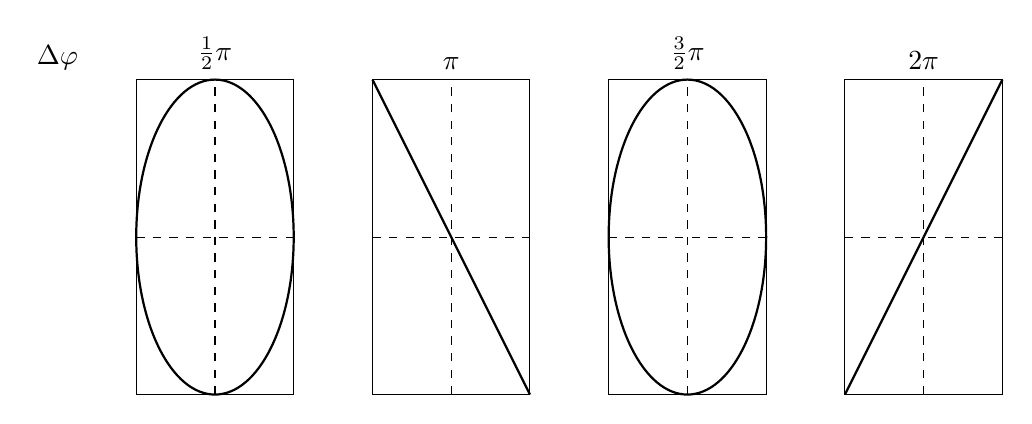
\begin{tikzpicture}
			\draw [thick] (0,0) ellipse (1 and 2);
			\draw (-1,-2) rectangle (1,2);
			\draw [dashed] (-1,0)--(1,0);
			\draw [dashed] (0,-2)--(0,2);
			\node [above] at(0,2) {$ \frac12\pi $};
			
			\draw [thick] (2,2) -- (4,-2);
			\draw (2,-2) rectangle (4,2);
			\draw [dashed] (2,0)--(4,0);
			\draw [dashed] (3,-2)--(3,2);
			\node [above] at(3,2) {$ \pi $};
			
			\draw [thick] (6,0) ellipse (1 and 2);
			\draw (5,-2) rectangle (7,2);
			\draw [dashed] (5,0)--(7,0);
			\draw [dashed] (6,-2)--(6,2);
			\node [above] at(6,2) {$ \frac32\pi $};
			
			\draw [thick] (8,-2) -- (10,2);
			\draw (8,-2) rectangle (10,2);
			\draw [dashed] (8,0)--(10,0);
			\draw [dashed] (9,-2)--(9,2);
			\node [above] at(9,2) {$ 2\pi $};
			
			\node [above] at(-2,2) {$ \Delta\varphi $};
		\end{tikzpicture}
		\caption{频率相同、相位差变化时的李萨如图形}
	\end{figure}

	\subsection{声速的理论值}
	利用声速在空气中的理论公式可以计算空气中声速的理论值:
	\[v=v_0\sqrt{\frac{T}{T_0}}=v_0\sqrt{1+\frac{t}{273.15}}\]
	其中$ T=(t+273.15)\,\mathrm K $,$ t $为摄氏温度,$ v_0=331.45\,\mathrm{m/s} $为$ 0 $\,\textcelsius 时的声速。
	
	\section{实验内容}
	1.利用驻波法测超声波在空气中的波速;
	
	2.利用相位法测超声波在空气中的波速;
	
	3.利用驻波法或相位法测超声波在水中的波速;
		
	4.利用逐差法处理实验数据。
	
	\section{实验结果与数据处理}
	\subsection{驻波法测超声波在空气中的声速}
	实验时室温为$ t=24.0 $\,\textcelsius,调节信号发生器产生频率$ f=38\,\mathrm{kHz} $的正弦波,连接实验器材,调节声速测量仪鼓轮,用驻波法测量得到数据如下:
	\begin{table}[!h]
		\centering
		\renewcommand\arraystretch{1.4}
		\captionsetup{skip=0pt}
		\caption{驻波法测定超声波在空气中的声速}
		\begin{tabularx}{\textwidth}{|c|Y|Y|Y|Y|Y|}
			\hline
			\textbf{序号}$ i $&\textbf{1}&\textbf{2}&\textbf{3}&\textbf{4}&\textbf{5}\\
			\hline
			\textbf{驻波法}$ L_i $(mm)&41.376&46.242&50.800&55.634&60.042\\
			\hline
			\textbf{序号}$ i $&\textbf{6}&\textbf{7}&\textbf{8}&\textbf{9}&\textbf{10}\\
			\hline
			\textbf{驻波法}$ L_i $(mm)&65.018&69.786&74.338&78.918&83.646\\
			\hline
		\end{tabularx}
	\end{table}
	
	利用逐差法处理上表数据可求得波长$ \lambda $为
	\[\lambda=\frac{\sum_{i=1}^{5}2(L_{i+5}-L_i)/5}{5}=9.40896\,\mathrm{mm}=9.40896\times10^{-3}\,\mathrm{m}\]
	故而根据$ v=\lambda f $可求得波速为
	\[v=357.54\,\mathrm{m/s}\]
	
	又根据实验原理部分可计算得到理论推导的理论波速为
	\[v_{\text{理}}=v_0\sqrt{1+\frac{t}{273.15}}=345.70\,\mathrm{m/s}\]
	故而实验结果与理论波速的相对误差为3.4349\%.
	
	\subsection{相位法测超声波在空气中的声速}
	室温与超声波与上小节相同,用相位法取$ \Delta\varphi=\pi,2\pi $时的位置测得数据如下:
	\begin{table}[!h]
		\centering
		\renewcommand\arraystretch{1.4}
		\captionsetup{skip=0pt}
		\caption{相位法测定超声波在空气中的声速}
		\begin{tabularx}{\textwidth}{|c|Y|Y|Y|Y|Y|}
			\hline
			\textbf{序号}$ i $&\textbf{1}&\textbf{2}&\textbf{3}&\textbf{4}&\textbf{5}\\
			\hline
			\textbf{相位法}$ L_i $(mm)&30.792&35.638&40.054&44.750&49.360\\
			\hline
			\textbf{序号}$ i $&\textbf{6}&\textbf{7}&\textbf{8}&\textbf{9}&\textbf{10}\\
			\hline
			\textbf{相位法}$ L_i $(mm)&53.968&58.490&63.200&67.102&71.970\\
			\hline
		\end{tabularx}
	\end{table}

	利用逐差法处理上述数据可求得波长$ \lambda $为
	\[\lambda=\frac{\sum_{i=1}^{5}2(L_{i+5}-L_i)/5}{5}=9.13088\,\mathrm{mm}=9.13088\times10^{-3}\mathrm m\]
	故而根据$ v=\lambda f $求得波速为
	\[v=346.97\,\mathrm{m/s}\]
	由于室温未发生改变,复用上小节求得的理论波速\[ v_{\text{理}}=345.70\,\mathrm{m/s} \]故而实验值与理论值的相对误差为0.3674\%.
	
	\subsection{相位法测超声波在水中的声速}
	调节信号发生器产生频率$ f=1.8\,\mathrm{MHz} $的正弦波,连接实验器材,调节声速测量仪鼓轮,用相位法取$ \Delta\varphi=2\pi $时的位置测得数据如下:
	\newpage
	\begin{table}[!h]
		\centering
		\renewcommand\arraystretch{1.4}
		\captionsetup{skip=0pt}
		\caption{相位法测定超声波在水中的声速}
		\begin{tabularx}{\textwidth}{|c|Y|Y|Y|Y|Y|}
			\hline
			\textbf{序号}$ i $&\textbf{1}&\textbf{2}&\textbf{3}&\textbf{4}&\textbf{5}\\
			\hline
			\textbf{相位法}$ L_i $(mm)&40.792&41.498&42.564&43.530&44.300\\
			\hline
			\textbf{序号}$ i $&\textbf{6}&\textbf{7}&\textbf{8}&\textbf{9}&\textbf{10}\\
			\hline
			\textbf{相位法}$ L_i $(mm)&45.144&45.928&46.766&47.500&48.384\\
			\hline
		\end{tabularx}
	\end{table}

	利用逐差法处理上表数据可求得波长$ \lambda $为
	\[\lambda=\frac{\sum_{i=1}^{5}(L_{i+5}-L_i)/5}{5}=0.84152\times10^{-3}\,\mathrm{m/s}\]
	故而根据$ v=\lambda f $可求得波速为
	\[v=1514.736\,\mathrm{m/s}\]
\end{document}